\documentclass[
%% TIKZ_CLASSOPTION %%
tikz
]{standalone}
\usepackage{amsmath}
\usetikzlibrary{matrix}
%% EXTRA_TIKZ_PREAMBLE_CODE %%
\begin{document}
%% TIKZ_CODE %%
\usetikzlibrary{decorations.pathreplacing,angles,quotes}
\colorlet{DarkGreen}{green!40!black!60}
\colorlet{LightBlue}{blue!60!white!40}
\colorlet{LightRed}{red!40!white!60}
\colorlet{DarkRed}{red!40!black!60}
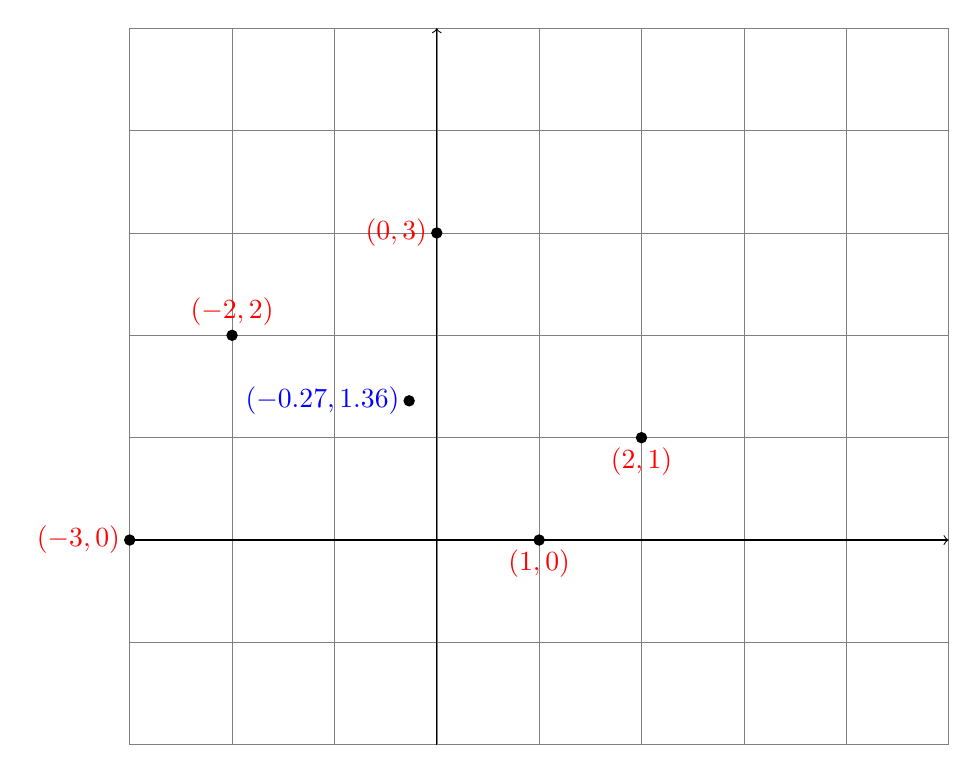
\begin{tikzpicture}[scale=1.3]
  \draw[step=1cm,gray,very thin] (-3,-2) grid (5,5);
  \draw [<-] (0,5) -- (0,-2);
  \draw [->] (-3,0) -- (5,0);
  \draw[fill] (1,0) circle [radius=0.05];
  \node [red, below] at (1,0) {$(1,0)$};
  \draw[fill] (2,1) circle [radius=0.05];
  \node [red, below] at (2,1) {$(2,1)$};
  \draw[fill] (-3,0) circle [radius=0.05];
  \node [red, left] at (-3,0) {$(-3,0)$};
  \draw[fill] (-2,2) circle [radius=0.05];
  \node [red, above] at (-2,2) {$(-2,2)$};
  \draw[fill] (0,3) circle [radius=0.05];
  \node [red, left] at (0,3) {$(0,3)$};
  \draw[fill] (-0.27,1.36) circle [radius=0.05];
  \node [blue, left] at (-0.27,1.36) {$(-0.27,1.36)$};
\end{tikzpicture}
\end{document}
